% Two slides for the 3-minute lightning presentation (due November 23, 2026).
% Build from docs/:  pdflatex slides.tex && pdflatex slides.tex
\documentclass{article}
\usepackage[paperwidth=33.867cm,paperheight=19.05cm,margin=0cm]{geometry}
\usepackage[T1]{fontenc}
\usepackage[sfdefault]{inter}
\usepackage{graphicx}
\usepackage{xcolor}
\usepackage{tikz}
\usepackage{microtype}
\pagestyle{empty}
\setlength{\parindent}{0pt}

\definecolor{paper}{HTML}{FBFBF8}
\definecolor{ink}{HTML}{0B0B0B}
\definecolor{muted}{HTML}{52514E}
\definecolor{rule}{HTML}{D9D8D3}
\definecolor{blue}{HTML}{2A78D6}
\definecolor{red}{HTML}{E34948}
\definecolor{grey}{HTML}{A8A7A1}
\pagecolor{paper}
\color{ink}

\newcommand{\fs}[2]{\fontsize{#1}{#2}\selectfont}
\newcommand{\kicker}[1]{{\fs{13}{16}\bfseries\color{blue}\MakeUppercase{#1}}}
\newcommand{\at}[3][]{\node[anchor=north west,inner sep=0pt,#1] at ([xshift=#2,yshift=-#3]current page.north west)}

\begin{document}

% ---------------------------------------------------------------- slide 1
\begin{tikzpicture}[remember picture,overlay]
\at{1.6cm}{1.2cm}{\parbox{30cm}{\fs{30}{36}\bfseries Snake-like bodies evolved dozens of times.\\ Where do unrelated lizards converge?}};
\at{1.6cm}{3.95cm}{\parbox{30cm}{\fs{15}{18}\color{muted}Henry Ji and Calvin Zhang \quad\textperiodcentered\quad CS/INFO 6850 project preview}};

\at{1.6cm}{5.5cm}{\parbox{16.9cm}{\raggedright
\kicker{The puzzle}\\[3pt]
{\fs{16.5}{23}Long trunk, reduced or lost limbs: a rare body form that keeps reappearing in lizard lineages separated by over 100 million years.\par}
\vspace{15pt}
\kicker{Prior work}\\[3pt]
{\fs{16.5}{23}Biology follows traits along the evolutionary tree: correlated traits (Pagel 1994), walks on the hypercube of trait combinations (HyperTraPS, 2020), several routes to a snake-like form (Bergmann \& Morinaga 2019).\par}
\vspace{15pt}
\kicker{Our angle}\\[3pt]
{\fs{16.5}{23}Make the species themselves a network and ask the course's questions: is it a small world, where is its thinnest cut, where do random walks go?\par}
}};

\at{19.6cm}{4.9cm}{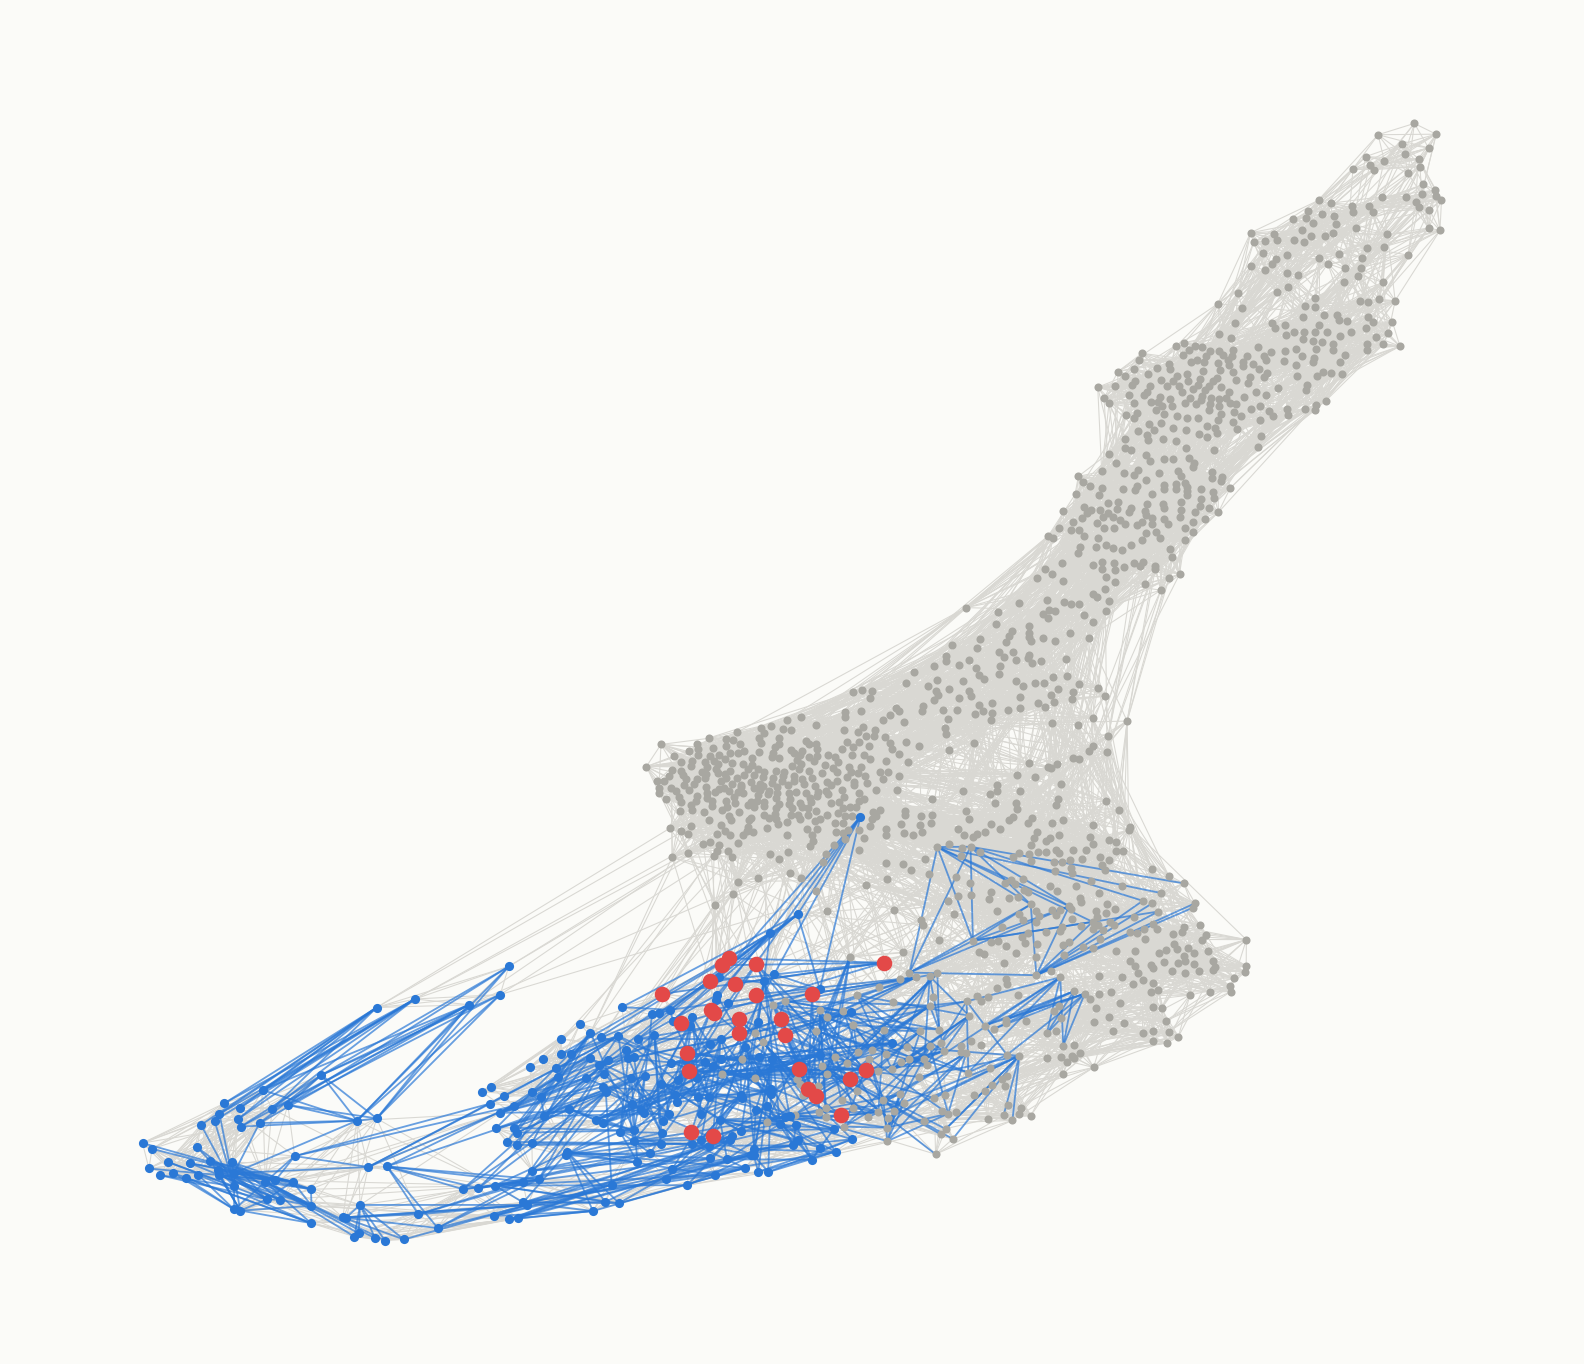
\includegraphics[height=11.6cm]{../results/species_network_drawing.png}};
\at{19.9cm}{5.5cm}{\parbox{7.6cm}{\raggedright\fs{14}{19}%
\textbf{1,451 lizard species}\\
each linked to its 6 closest relatives and its 6 closest look-alikes}};
\at{19.4cm}{16.8cm}{\parbox{14.2cm}{\raggedright\fs{12}{18}\color{muted}%
{\color{grey}\rule[0.5pt]{9pt}{9pt}}\; limbed \quad
{\color{blue}\rule[0.5pt]{9pt}{9pt}}\; snake-like \quad
{\color{red}\rule[0.5pt]{9pt}{9pt}}\; bridge \quad
{\color{blue}\rule[3.5pt]{16pt}{1.6pt}}\; convergence link\\
Data: five trait sources merged on the Title et al.\ (2024) dated tree}};
\end{tikzpicture}
\newpage

% ---------------------------------------------------------------- slide 2
\begin{tikzpicture}[remember picture,overlay]
\at{1.6cm}{1.3cm}{\parbox{30.6cm}{\fs{30}{36}\bfseries One thin cut separates snake-like lizards from the rest}};
\at{1.6cm}{2.85cm}{\parbox{30.6cm}{\fs{15}{20}\color{muted}Cheeger sweep cut of the Fiedler vector, on the graph linking species by similarity of body form}};

\at{1.1cm}{4.5cm}{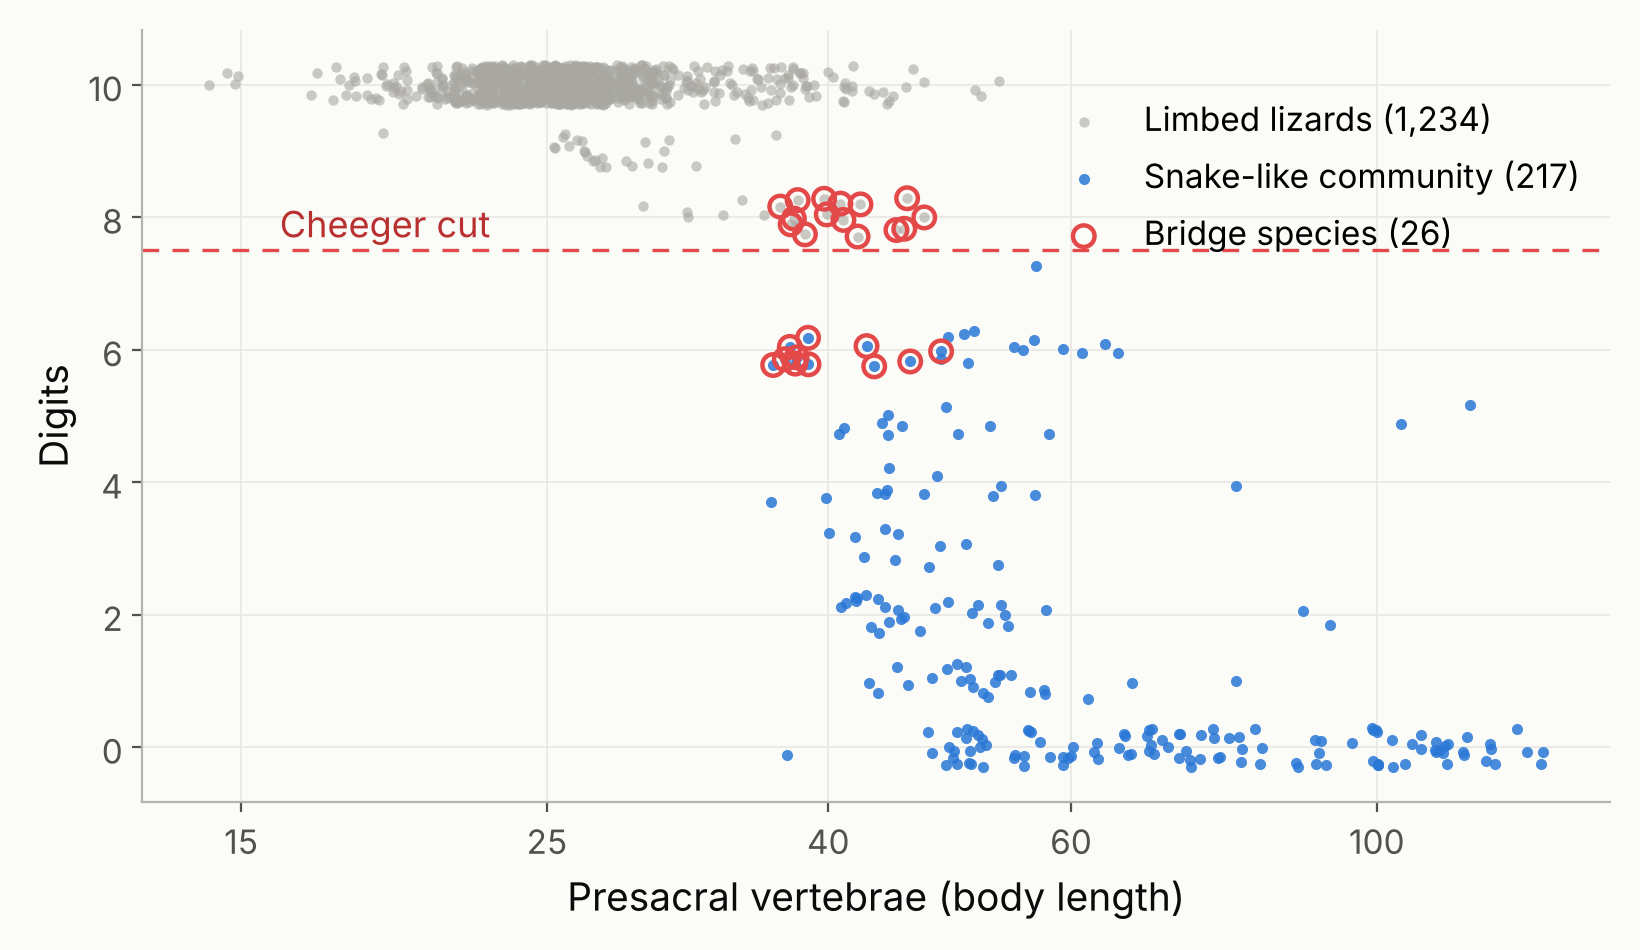
\includegraphics[width=20.6cm]{../results/slide_cut.png}};

\at{22.9cm}{4.7cm}{\parbox{9.6cm}{\raggedright
{\fs{32}{36}\bfseries\color{blue}0.003}\\[4pt]
{\fs{15}{20.5}conductance of the cut\\ {\color{muted}(95\% interval 0.002--0.004);\\ the next-best cut found: 0.38}\par}
\vspace{15pt}
{\fs{32}{36}\bfseries\color{blue}30}\\[4pt]
{\fs{15}{20.5}separate lineages on the snake-like side {\color{muted}(split over 50 Myr ago; 217 species, 15 families)}: convergence\par}
\vspace{15pt}
{\fs{32}{36}\bfseries\color{red}26}\\[4pt]
{\fs{15}{20.5}bridge species span it: \textit{Lerista}, \textit{Brachymeles}, \textit{Bachia}, the genera biologists already study for limb loss\par}
}};

\draw[rule,line width=0.8pt] ([xshift=1.6cm,yshift=-17.0cm]current page.north west) -- ++(30.6cm,0);
\at{1.6cm}{17.4cm}{\parbox{30.6cm}{\raggedright\fs{14}{19}\color{muted}%
Same cut in 200 of 200 subsamples of the species, and in a second dataset and tree with every digit directly counted.\quad
\textcolor{ink}{Next: why it is so thin.} Walks on the dated tree suggest the change is hard to start and quick to finish.}};
\end{tikzpicture}

\end{document}
